\documentclass{article}

\usepackage[a4paper]{geometry}
\usepackage{fancyhdr}
\usepackage{graphicx}
\usepackage{listings}
\usepackage{textcomp}
\usepackage{hyperref}
\usepackage{lastpage}

\graphicspath{{img/}}

\AddToHook{cmd/section/before}{\newpage}

\def\Title{Early Earthquake and Tsunami Warning Viewer}
\def\Author{Yicheng Shao (Eason)}
\def\CandNo{Insert\_Candidate\_Number\_Here}

\title{\Title}
\author{\Author}
\date{\today}

\fancypagestyle{nohead}{
    \renewcommand{\headrulewidth}{0pt}
    \fancyhf{}
    \lfoot{\CandNo}
    \rfoot{Page \thepage\ of \pageref{LastPage}}
}

\begin{document}
\pagestyle{fancy}

\maketitle
\subsection*{Abstract}
Give a brief summary outline of your project.
\thispagestyle{nohead}

\newpage
\noindent \copyright 2025 Y. Shao. This work is licensed under \href{https://creativecommons.org/licenses/by-nc-nd/4.0/}{CC BY-NC-ND 4.0}. To view a copy of this license, visit https://creativecommons.org/licenses/by-nc-nd/4.0/.
\thispagestyle{nohead}

\newpage
\tableofcontents
\thispagestyle{nohead}

\fancyhf{}
\lhead{\Author}
\rhead{\Title}
\lfoot{\CandNo}
\rfoot{Page \thepage\ of \pageref{LastPage}}

\section{Analysis}

\subsection{Background Information}

\subsubsection{The Early Earthquake Warning System}

Earthquake is one of the most common natural disasters in the whole world, and direct consequences of earthquakes include tsunamies which could be catastrauphic.

Japan, sitting on the intersection of the Eurasian, the Philippine and the North-American plates, is the countries with most earthquakes. Historically, the Great Kant\=o Earthquake in 1923, the Great East Japan Earthquake in 2011 (a.k.a. the T\=ohoku Earthquake) and the recent 2024 Noto Peninsula Earthquake all caused hundreds of deaths, both due to the result of the earthquake(s) and the resulting tsunami.

To provide protection to its residents, the Japan Meterological Agency (JMA), together with the National Research Institute for Earth Science and Disaster Resilience (NIED) placed thousands of \textbf{earthquake sensors} across Japan (the Hi-net), with several lying deep in the sea bed, measuring displacement, velocity and acceleration, which are connected to multiple servers, including two located in \=Osaka and T\=okyo.

Using data obtained from the sensors, computers do some complicated algorithms (mentioned below) to send out \textbf{early earthquake warnings (EEWs)} automatically within milliseconds. There are two types of EEWs:
\begin{enumerate}
    \item \textbf{EEW (Forecast).} Sent out to \textbf{highly-dependent industries} (e.g. rail industry, power plants) and \textbf{subscribed users}, when maximum intensity level of more than 3, or a magnitude of more than 3.5 is expected.
    \item \textbf{EEW (Warning).} Sent out to \textbf{everyone} via TV, Radio, Mobile Phone, SMS, etc., when a maximum intensity level of more than 4 is expected.
\end{enumerate}

After the earthquake, JMA staff will determine the location and severity of tsunami warnings to be issued, if necessary.

\subsubsection{Earthquake Terminology}

\begin{itemize}
    \item \textbf{Intensity.} The intensity describes the intensity vibration of a point due to an earthquake. It is not unique to an earthquake - \textbf{different places can have different intensities} due to the distance to the epicenter, and intensity will also change over time. JMA measures intensity using \textbf{9 levels: 1, 2, 3, 4, 5--, 5+, 6--, 6+ and 7} in increasing order.
    \item \textbf{Magnitude/Scale.} The magnitude of an earthquake describes the energy released in the earthquake in a logarithmic scale. \textbf{It is unique to an earthquake.}
    \item \textbf{Epicenter/Hypocenter.} The epicenter is the surface point directly above the true centre of the earthquake.
    \item \textbf{Focal Depth.} The focal depth is the depth of the true center of the earthquake.
    \item \textbf{P-Wave and S-Wave.} These are seismic waves, sourced from the true center of the earthquake, travelling at different speeds, with Primary (P)-Wave travelling faster and Secondary (S)-Wave travelling slower.
\end{itemize}

\subsection{Problem Area}
The main goal of this application is to provide a visuallisation of the earthquake/tsunami related data feed(s) provided by JMA's affliated institution, Disaster Migitation Data Send Service (DM-D.S.S). There are numerous seperate apps providing a list of recent earthquakes, the real-time data measured by the sensors, and the real time earthquake warning displayed on a map, but rarely are there good apps that combine all those features together in a satisfying way, with just the necessary features I need.

Some applications are no longer being updated due to change in the user's policy of the related data feed. Furthermore, most of the apps avaliable are only in Japanese, not in English or my home language Chinese, which can create trouble for me to understand.

\subsection{Client and End User}
The primary target of this application will be passionate geographers and geologists who are interested in the study of earthquake obserations and predictions. The age group of this vary all the way from primary-school students to adults, including me who has been amazed by the technology since the age of 12. They could take any employment, ranging from students to full-time jobs. Their proficiency usually varies, since there are people new to this field who probably does not have much knowledge, so the interface of the applciation should be relatively user-friendly and understandable, hiding unnessary technical complexities.

Another target client could be industries which highly rely on earthquake predictions due to the risk imposed by earthquakes. High-speed railway and nuclear power plants are good examples of this. Therefore, the staff in charge monitoring will usually have higher proficiency and would like more detailed data of the earthquake. However, they will only need the necessary data from earthquakes happening close to them and only require intensity data of the point in interest (e.g. the power plant). To put this into content, an earthquake happening 1000km away from them does not need to be fed into their system, while they would like to see the intensity of the shock and the arrival time of the seismic waves to decide the actions.

\subsection{Research Methodology}
Describe \textbf{how} you went about investigating the requirements. This may include a range of measures:
\begin{itemize}
    \item Investigation of similar systems
    \item Web research for key concepts/algorithms
    \item Client/end user interview
    \item Questionnaires to potential end-users of the system
\end{itemize}

\subsection{Features of proposed solution}
As a result of research, you should identify the key features (in general terms) that your system will have:
\begin{itemize}
    \item List of key features that will be Required
    \item Discussion of the scope and potential limitations to the system given the time constraints.
\end{itemize}

\subsection{Requirements Specification}
The requirements specification is a document/contract with the client that outlines what you will deliver. The contents need to have SMART (specific, measurable, achievable, realistic, timely) goals.

After your system has been completed you will need to test against this.

\begin{table}[!ht]
    \centering
    \begin{tabular}{|l|p{0.15\linewidth}|l|p{0.3\linewidth}|}
        \hline
        Requirement \textnumero & Description & Success Criteria & Measurement Method \\
        \hline \hline
         & & &\\
        \hline
         & & &\\
        \hline
         & & & \\
        \hline
    \end{tabular}
    \caption{Table of Requirements.}
    \label{table:requirements}
\end{table}

\subsection{Critical Path}

Order of development for the tasks that will need to be completed. This may reflect an iterative approach to software development. Software development will be undertaken using an \textit{agile} methodology as opposed to a \textit{waterfall} model of software development. It is expected that development will go through a number of iterations that will add increasing functionality to the system.

\section{Design}
Algorithms + Data Structures = Programs.

\subsection{Hierarchy Chart}
A top-down approach to problem solving will lead to the identification of tasks with sub-tasks. i.e. modules and functions required. This shows how \textbf{decomposition} is applied.

\begin{figure}[!ht]
    \centering
    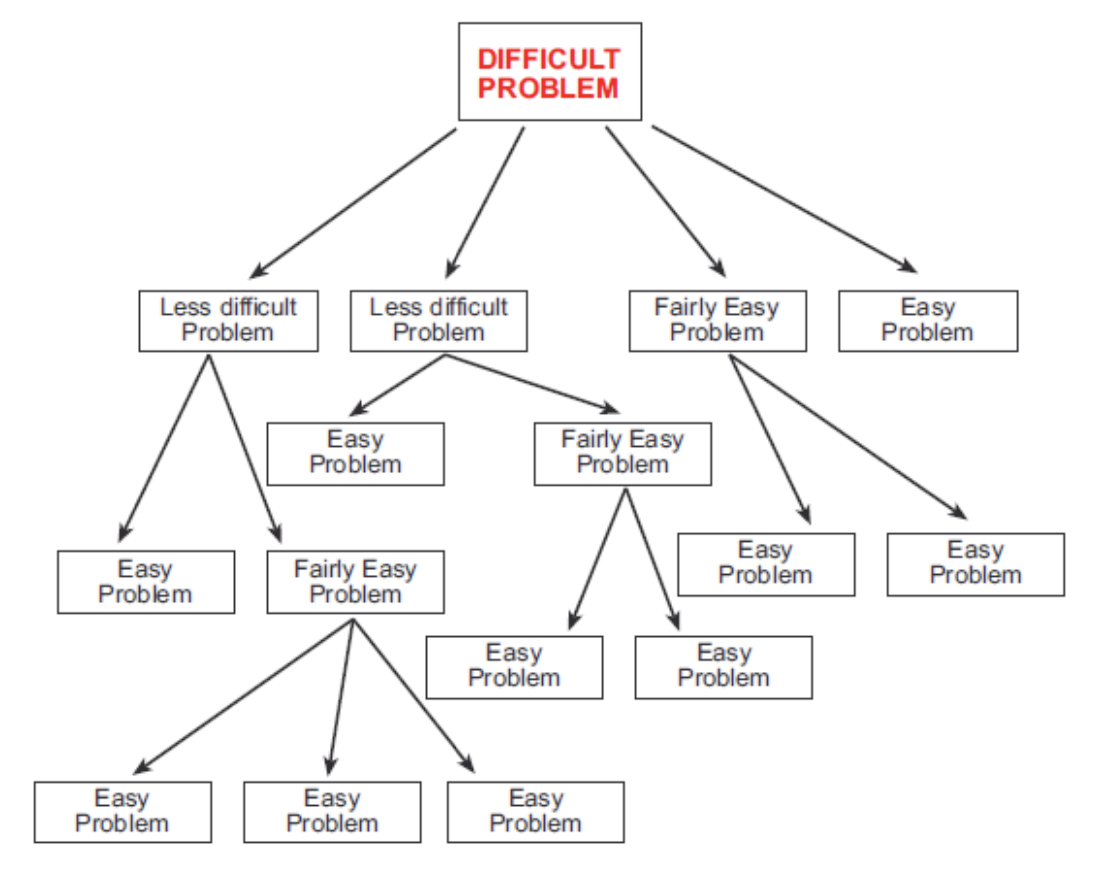
\includegraphics[width = 0.5\linewidth]{hierarchy_chart.png}
    \caption{Hierarchy Chart.}
    \label{fig:hierarchy}
\end{figure}

\subsection{Data Structures/Data modelling}
\subsubsection{External Data Sources}
If you are scraping/gathering data from APIs from external sources you should define the relevant format/parameters.

\subsubsection{OOP Model}
OOP modelling (classes, methods, attributes, inheritance etc.). Class diagrams would be useful (these are covered in Bond book 1 page 185 onwards). Diagrams should follow conventions for inheritance/composition and private/protected/public methods/attributes.

\begin{figure}[!ht]
    \centering
    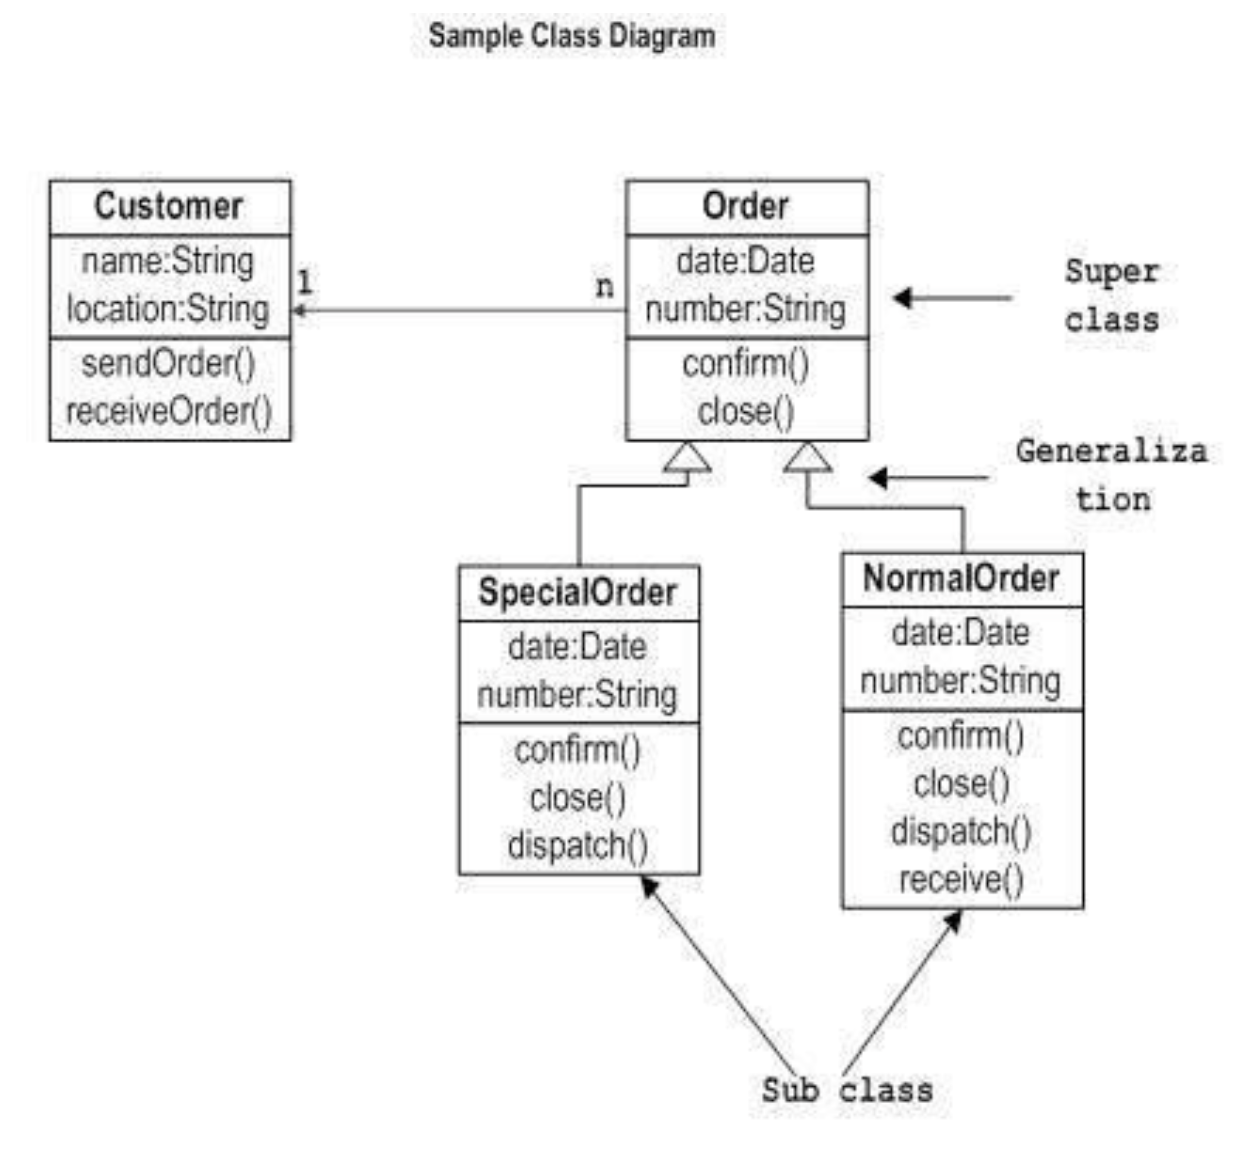
\includegraphics[width = 0.5\linewidth]{class_diagram.png}
    \caption{Class Diagram.}
    \label{fig:classes}
\end{figure}

\subsection{User Interface}
You will need to draw up a prototype for the user interface. You may do this within the software package you implement your solution in.
\begin{itemize}
    \item Screen designs
    \item Menu options/sequences
    \item Buttons/keys/commands (command line)
\end{itemize}

\subsection{Hardware \and Software Requirements}
Draw up a hardware and software specification for items that are required.

\section{Technical Implementation}
\subsection{Key Code Segments}
\subsubsection{Data structures}
Implementation of ADTs and OOP Classes to be demonstrated.

\subsubsection{Modularity}
Code should be created and tested in separate modules that are integrated later. Use sub-headings for each module, define the purpose of the module, and show unit testing of the module.

\subsubsection{Defensive Programming/Robustness}
Exception handling

\section{Testing}
Consider how you will test your project. You should devise a test strategy that encompasses a range of methods.

\subsection{Test Strategy}
\begin{itemize}
    \item Unit testing (of individual functions)
    \item Integration testing (e.g. different modules/class files)
    \item Robustness (demonstrating defensive programming skills/exception handling)
    \item Requirements testing (against your initial requirements - a table with test number, description, test data, expected result, evidence (screenshot/video time link) would be suitable)
    \item Independent end user beta testing (this will assist with your evaluation)
\end{itemize}

\subsection{Testing Video}
\begin{itemize}
    \item You can include a video to assist (but you will need to reference the timepoint at which relevant evidence appears)
    \item If you include a video you will need to have it publicly available.
    \item It is suggested that you include a QR code in your testing to give a link to it the video (for the moderator) rather than just giving a long URL on its own.
\end{itemize}

\subsection{System Tests (against original requirements specification)}
You need to give evidence in support of requirements that have been met e.g. reference to a relevant test/screenshot/relevant code.

\begin{table}[!ht]
    \centering
    \begin{tabular}{|l|p{0.15\linewidth}|l|p{0.3\linewidth}|}
        \hline
        Requirement \textnumero & Description & Success Criteria & Tests + Evidence \\
        \hline \hline
         & & &\\
        \hline
         & & &\\
        \hline
         & & & \\
        \hline
    \end{tabular}
    \caption{Table of Tests.}
    \label{table:tests}
\end{table}

\section{Evaluation}
\subsection{Requirements Specification Evaluation}
Personal evaluation
\begin{itemize}
    \item Copy and paste your original requirements from your project analysis
    \item You need to review each requirement and comment objectively on whether it was \textit{fully met/partially met/not met}.
\end{itemize}

\begin{table}[!ht]
    \centering
    \begin{tabular}{|l|p{0.15\linewidth}|l|p{0.3\linewidth}|}
        \hline
        Requirement \textnumero & Description & Success Criteria & Fully/Partial/Not met (Reflective Comment) \\
        \hline \hline
         & & &\\
        \hline
         & & &\\
        \hline
         & & & \\
        \hline
    \end{tabular}
    \caption{Table of Evaluation.}
    \label{table:evaluation}
\end{table}

\subsection{Independent End-User Feedback}
End user/client evaluation
\begin{itemize}
    \item there \textbf{must} be meaningful end user feedback
    \item You should hold a review meeting with your end user
    \item Write down any key feedback that they give you. E.g. Agreement that a particular requirement has been meet/comments as to aspects that they find sub-optimal/comments as to additions they would like to see
\end{itemize}

\begin{table}[!ht]
    \centering
    \begin{tabular}{|l|p{0.15\linewidth}|l|p{0.3\linewidth}|}
        \hline
        Requirement \textnumero & Description & Acceptance Y/N & Additional Comments \\
        \hline \hline
         & & &\\
        \hline
         & & &\\
        \hline
         & & & \\
        \hline
    \end{tabular}
    \caption{Table of Feedback.}
    \label{table:feedback}
\end{table}

\subsection{Improvements}

You need to give consideration to a number of potential future improvements that could be made. They may arise from either your experience or from feedback given to you by your end user. Ideally at least one should be in response to end user feedback.

\begin{itemize}
    \item Write a paragraph for each potential improvement/change
    \item The improvements/changes could result from additional functionality that has been identified as being beneficial or could be as a result of required efficiencies if some processes are clunky or require faster run-times
    \item You should then comment on how the proposed change could be implemented moving forward. i.e. what would need to be changed/developed and how? You are not expected to actually make any changes; just comment on the possibilities.
\end{itemize}

\section{Code Listing}


\end{document}